\chapter{Cơ sở Lý thuyết}
\label{ch:theoretical_background}

Chương này thiết lập các nền tảng lý thuyết và cơ sở khoa học chuyên sâu làm chỗ dựa vững chắc cho việc thiết kế và triển khai hệ thống SENTINEL. Trọng tâm nghiên cứu được triển khai mạch lạc thông qua cấu trúc phân tầng logic: bắt đầu bằng việc mổ xẻ các nút thắt nhận thức và hiện tượng quá tải thông tin tại các Trung tâm Điều hành An ninh (SOC) hiện đại; tiếp nối bởi nền tảng toán học của việc tối ưu hóa hiệu năng suy luận thông qua lượng tử hóa Mô hình Ngôn ngữ Lớn (LLM) cục bộ; phân tích cơ chế điều phối có trạng thái của kiến trúc AI Tác tử (Agentic AI) dựa trên đồ thị có hướng; cơ chế củng cố tri thức chuyên ngành bằng giải pháp Sinh tăng cường Truy xuất (RAG) lai; nhận diện các vector tấn công đối kháng đặc thù nhắm vào LLM trong môi trường xử lý log; và cuối cùng là toán học hóa thuật toán thống kê trực tuyến Welford phục vụ lọc dữ liệu tốc độ cao và mô phỏng đe dọa zero-day thực tế.

\section{Tổng quan về Trung tâm Điều hành An ninh (SOC) và Nút thắt Nhận thức}

Các Trung tâm Điều hành An ninh (SOC) đóng vai trò là tuyến phòng thủ hạt nhân trong việc bảo vệ hạ tầng công nghệ thông tin của doanh nghiệp, thực hiện giám sát thông qua việc hợp nhất luồng dữ liệu đo lường từ xa từ các thiết bị tường lửa thế hệ mới (NGFW), hệ thống giám sát điểm cuối (EDR) và các cảm biến phân tích lưu lượng mạng (IDS/IPS). Quy trình xử lý sự cố tiêu chuẩn đòi hỏi sự tập trung hóa các nguồn nhật ký này về các nền tảng Quản lý Thông tin và Sự kiện An ninh (SIEM)~\cite{siem2021} nhằm mục đích chuẩn hóa dữ liệu, đối sánh tương quan và chuyển tiếp các sự kiện nghi vấn đến các chuyên viên phân tích để điều tra và xử lý.

Tuy nhiên, sự bùng nổ của hạ tầng điện toán đám mây và các dịch vụ phân tán đã làm gia tăng quy mô của dữ liệu nhật ký mạng theo cấp số nhân~\cite{bigdata2019}. Việc gia tăng lưu lượng telemetry này trực tiếp gây ra hội chứng bội thực cảnh báo hệ thống. Lực lượng phân tích tầng đầu tiên (Tier-1) thường xuyên đối mặt với khối lượng cảnh báo khổng lồ mỗi ngày, trong đó các trường hợp dương tính giả (false positives) chiếm tỷ lệ áp đảo. Hiện tượng cạn kiệt tài nguyên chú ý do dòng thác cảnh báo liên tục làm suy giảm đáng kể năng lực xử lý nhận thức của con người, từ đó gia tăng xác suất bỏ sót các hành vi xâm nhập thực sự nguy hiểm \cite{alertfatigue2022}.

\begin{figure}[!htbp]
    \centering
    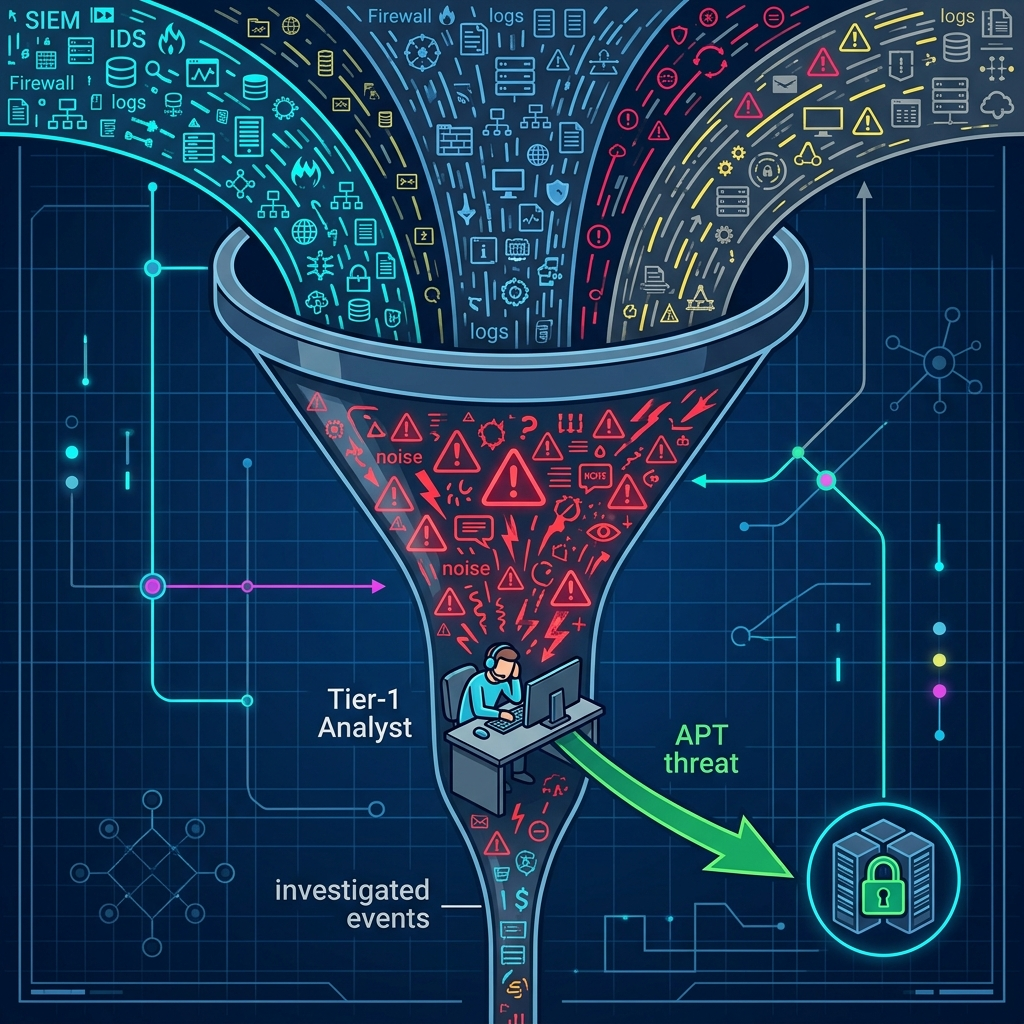
\includegraphics[width=0.85\textwidth]{images/soc_human_bottleneck.png}
    \caption{Nút thắt nhận thức ở con người trong các hệ thống SOC truyền thống khi đối mặt với khối lượng cảnh báo vượt quá khả năng xử lý. (Nguồn: Tác giả)}
    \label{fig:soc_bottleneck}
\end{figure}

Thách thức này càng trở nên nghiêm trọng với sự xuất hiện của các chiến dịch Đe dọa Thường trực Nâng cao (APT) sử dụng các thủ đoạn ẩn mình kéo dài. Các bộ quy tắc phát hiện tĩnh truyền thống không có khả năng tích lũy ngữ cảnh phiên dài hạn hoặc thiết lập mối tương quan giữa các hành vi rời rạc, khiến hệ thống dễ tổn thương trước các kỹ thuật thâm nhập chậm rãi và tinh vi \cite{apt_stealth2021}. Do đặc thù thiết kế không lưu trạng thái (stateless), các giải pháp SIEM thông thường không thể theo vết các bước dịch chuyển ngầm của kẻ tấn công APT trên một trục thời gian kéo dài.

\section{Mô hình Ngôn ngữ Lớn (LLM) và Cơ sở Toán học của Lượng tử hóa}

Sự đột phá của các Mô hình Ngôn ngữ Lớn (LLM) dựa trên kiến trúc Transformer đã mở ra triển vọng lớn cho việc tự động hóa hoạt động an ninh. Hiệu quả của chúng bắt nguồn từ cơ chế tự chú ý (self-attention), vốn cân nhắc song song mối liên hệ giữa mọi token với tất cả các token còn lại trong chuỗi \cite{vaswani2017}; nhờ đặc tính này, mô hình nắm bắt được các phụ thuộc tầm xa cần thiết để đối chiếu những sự kiện nằm rải rác trong một luồng nhật ký kéo dài.

Mặc dù vậy, việc ứng dụng LLM trong môi trường SOC bị ràng buộc chặt chẽ bởi các nguyên tắc về chủ quyền dữ liệu. Việc chuyển tiếp dữ liệu đo lường mạng nội bộ nhạy cảm đến các máy chủ đám mây của bên thứ ba vi phạm nghiêm trọng các quy định tuân thủ bảo mật và kiến trúc an ninh không tin cậy (Zero Trust)~\cite{nist80207}, đặt ra yêu cầu bắt buộc phải vận hành các mô hình LLM cục bộ (Local LLM) trong môi trường mạng cách ly (air-gapped).

Bên cạnh đó, việc thực thi các mô hình có quy mô hàng tỷ tham số tại chỗ đòi hỏi tài nguyên phần cứng cực kỳ lớn. Ví dụ, vận hành mô hình \textit{Gemma-2-9B-IT} với kích thước 9 tỷ tham số ở định dạng số thực dấu phẩy động 16-bit (FP16) cần tối thiểu khoảng 18GB dung lượng bộ nhớ đồ họa (VRAM). Để hiện thực hóa khả năng suy luận trên các phần cứng thương mại phổ thông, kỹ thuật lượng tử hóa mô hình (Model Quantization) được áp dụng. Về bản chất, lượng tử hóa tái ánh xạ các trọng số liên tục có độ chính xác cao của mô hình (ví dụ số thực dấu phẩy động 16-bit) sang một lưới số nguyên thưa hơn với số bit thấp (ví dụ 4-bit), đánh đổi một mức mất mát độ chính xác có kiểm soát để tiết kiệm đáng kể bộ nhớ \cite{quantization2021}. Việc ứng dụng định dạng tập tin GGUF kết hợp tiêu chuẩn lượng tử hóa Q6\_K thông qua thư viện \texttt{llama.cpp} giúp giảm dung lượng bộ nhớ xuống còn khoảng 7--8\,GB VRAM (mức cắt giảm trên 50\%), tối đa hóa tốc độ xử lý suy luận trong khi vẫn bảo toàn được năng lực lập luận logic của mô hình. Bảng~\ref{tab:quantization} đối chiếu các mức lượng tử hóa liên quan cho mô hình 9 tỷ tham số và lý giải việc lựa chọn Q6\_K như một điểm cân bằng giữa dung lượng bộ nhớ và độ trung thực của suy luận.

\begin{table}[!htbp]
    \centering
    \caption{Các mức lượng tử hóa cho mô hình Gemma-2-9B (giá trị xấp xỉ). (Nguồn: Tác giả)}
    \label{tab:quantization}
    \begin{tabular}{|>{\raggedright\arraybackslash}p{0.26\textwidth}|>{\centering\arraybackslash}p{0.16\textwidth}|>{\centering\arraybackslash}p{0.16\textwidth}|>{\raggedright\arraybackslash}p{0.22\textwidth}|}
        \hline
        \textbf{Định dạng} & \textbf{Bit / trọng số} & \textbf{VRAM} & \textbf{Ảnh hưởng chất lượng} \\
        \hline
        FP16 (cơ sở) & 16 & $\approx$18\,GB & Không (tham chiếu) \\
        \hline
        \textbf{Q6\_K (đề tài này)} & $\approx$6.6 & $\approx$7--8\,GB & Gần như không mất mát \\
        \hline
        Q4\_K\_M & $\approx$4.5 & $\approx$5--6\,GB & Suy giảm nhẹ \\
        \hline
    \end{tabular}
\end{table}

\section{Kiến trúc AI Tác tử (Agentic AI) và Mô hình Đồ thị Trạng thái}

Nhằm khắc phục những giới hạn của các công cụ phân tích tĩnh, hướng tiếp cận tự động hóa an ninh đang dịch chuyển từ các kịch bản vận hành cứng nhắc (Runbook Automation - RBA) sang hệ thống AI Tác tử tự trị, hai mô hình khác biệt căn bản về phương thức vận hành. Tự động hóa Kịch bản (RBA) dựa trên các quy tắc tĩnh được định nghĩa trước và những đoạn mã tất định để xử lý cảnh báo tuyến tính; cách tiếp cận này có hiệu năng cao nhưng hoàn toàn mù lòa trước các biến thể zero-day hoặc cấu trúc log biến động. Ngược lại, hệ thống AI Tác tử (Agentic AI) thể hiện tính tự trị nhận thức (bao gồm khả năng tự phản biện, lập kế hoạch đa bước và định tuyến ngữ cảnh linh hoạt) cho phép điều chỉnh quy trình điều tra một cách linh động dựa trên các kết quả phát hiện trung gian.

Các hệ tác tử tự trị này được thiết lập toán học dưới dạng các Đồ thị có hướng lưu trạng thái hoạt động như một Máy Trạng thái Hữu hạn (FSM), trong đó các nút đại diện cho các bước tính toán hoặc hành động nhận thức cụ thể trong hệ thống (chẳng hạn như truy vấn cơ sở tri thức CTI, thực hiện rà quét lỗ hổng hoặc sinh phương án phản phó) và các cạnh điều kiện định nghĩa luồng di chuyển trạng thái động dựa trên kết quả suy luận của LLM tại các nút xử lý trung gian.

\begin{figure}[!htbp]
    \centering
    
\includegraphics[width=0.85\textwidth]{images/agentic_fsm_workflow.png}
    \caption{Đồ thị trạng thái (DAG) của tác tử Tầng 2 SENTINEL khi phân tích sự cố an ninh: sáu node và không có vòng lặp, phản ánh đúng luồng LangGraph đã triển khai. (Nguồn: Tác giả)}
    \label{fig:fsm_workflow}
\end{figure}

Phương pháp điều phối đa tác tử có lưu giữ trạng thái \cite{langgraph2024} cho phép hệ thống duy trì bộ nhớ làm việc xuyên suốt qua các sự kiện kế tiếp, nhờ đó ngữ cảnh tích lũy từ những phán quyết trước có thể soi sáng cho các phán quyết sau. Dù mô hình này cũng cho phép tái phân tích theo vòng lặp trong phạm vi một sự kiện, SENTINEL cố ý chọn duyệt phi chu trình (acyclic) cho mỗi sự kiện nhằm bảo đảm tính tất định và khả năng kiểm toán, và lưu giữ trạng thái xuyên sự kiện trong Bộ nhớ Đe dọa thay vì lặp bên trong quá trình phân tích của một sự kiện.

\section{Sinh Tăng cường Truy xuất (RAG) và Tối ưu hóa Tìm kiếm Lai}

Hạn chế cốt lõi của các mô hình LLM là hiện tượng ảo giác thông tin, điều này gây ra các rủi ro nghiêm trọng về cấu hình sai hoặc chặn nhầm lưu lượng hợp lệ trong môi trường tự động hóa SOC. Kỹ thuật Sinh Tăng cường Truy xuất (RAG) \cite{rag2020} hóa giải vấn đề này bằng cách gắn một kho tri thức bên ngoài có thẩm quyền vào mô hình ngay tại thời điểm suy luận: thay vì chỉ trả lời từ bộ nhớ tham số, mô hình điều kiện hóa mỗi câu trả lời dựa trên các đoạn văn bản vừa được truy xuất, qua đó thu hẹp không gian phát sinh những khẳng định không có căn cứ.

Để tối ưu hóa độ chính xác của quá trình truy xuất thông tin, các hệ thống RAG hiện đại áp dụng chiến lược tìm kiếm lai (hybrid search) kết hợp hai phương pháp bổ trợ cho nhau: tìm kiếm vector dày đặc, vốn chuyển đổi dữ liệu phi cấu trúc thành các biểu diễn không gian đa chiều thông qua mô hình nhúng (như \texttt{all-MiniLM-L6-v2}) và sử dụng thư viện FAISS để tính toán độ tương đồng Cosine \cite{faiss2019} nhằm nắm bắt ngữ nghĩa của truy vấn; và tìm kiếm từ khóa thưa thớt, dựa trên thuật toán BM25 \cite{bm25_2009} để tính toán tần suất xuất hiện của các định danh kỹ thuật đặc thù (như mã số CVE, tên file hoặc địa chỉ IP) so với toàn bộ cơ sở tri thức.

Quy trình chuẩn hóa thứ hạng sử dụng phương pháp Reciprocal Rank Fusion (RRF) \cite{rrf2009} giúp tích hợp hai danh sách kết quả tìm kiếm trên thành một danh sách duy nhất có độ chính xác cao nhờ sự cân bằng giữa tính tương đồng ngữ nghĩa rộng và độ chính xác của từ khóa kỹ thuật cụ thể.

\section{Lỗ hổng Nhận thức LLM và Vector Tấn công Prompt Injection}

Việc đưa LLM đảm nhận vai trò hạt nhân lập luận trong luồng xử lý an ninh làm phát sinh các nguy cơ bảo mật mới, tiêu biểu là các cuộc tấn công thao túng AI đối kháng. Do đặc tính của LLM là tiếp nhận và xử lý trực tiếp ngôn ngữ tự nhiên mà không có ranh giới biên dịch rõ ràng giữa dữ liệu đầu vào và tập lệnh thực thi, mô hình rất dễ bị chiếm quyền điều khiển chỉ thị \cite{promptinjection2023}.

Kiến trúc suy luận của hệ thống đối mặt với nguy cơ thao túng nghiêm trọng thông qua hình thức tiêm prompt từ log (log-substrate prompt injection) \cite{watchtower2026}. Ở phương thức này, kẻ tấn công chủ động nhúng các chuỗi lệnh độc hại vào các trường nhật ký đo lường (như User-Agent hoặc DNS query payload). Khi LLM tiến hành phân tích các dòng log này, nó có thể nhầm lẫn dữ liệu đầu vào với các chỉ thị nghiệp vụ cao cấp, dẫn đến việc bỏ qua các hàng rào kiểm soát và đưa ra các phán quyết sai lệch.

Các nghiên cứu gần đây hệ thống hóa các tấn công tiêm prompt từ log thành một phân loại bốn lớp \cite{watchtower2026}. Một tải trọng \textit{Ghi đè trực tiếp} (S1) yêu cầu mô hình bỏ qua trực tiếp các chỉ thị an toàn trước đó và ghi đè hướng dẫn hệ thống. Một tải trọng \textit{Chiếm vai trò} (S2) cưỡng ép mô hình chấp nhận một vai trò không bị giới hạn hoặc không được ủy quyền nhằm vượt qua ranh giới an toàn. Một tải trọng \textit{Thao túng ngữ cảnh} (S3) giả mạo thông tin xác thực hoặc nguồn gốc giả trong luồng log, ví dụ, tuyên bố rằng một cảnh báo đã được phê duyệt trước hoặc nằm trong whitelist. Cuối cùng, một \textit{Payload ngụy trang} (S4) che giấu chỉ thị độc hại bằng mã hóa Base64, thập lục phân hoặc URL, hoặc bằng ký tự đồng hình, nhằm vượt qua các bộ lọc regex tĩnh. Vì các trường log mang payload này do kẻ tấn công kiểm soát nhưng lại không thể phân biệt về mặt cấu trúc với bằng chứng hợp lệ, một LLM phân tích một-lượt không thể tách tin cậy dữ liệu khỏi chỉ thị. Phân loại này trực tiếp thúc đẩy thiết kế rào chắn phòng thủ nhiều lớp (defense-in-depth) được trình bày ở Chương~\ref{ch:system_design_implementation}.

\begin{figure}[!htbp]
    \centering
    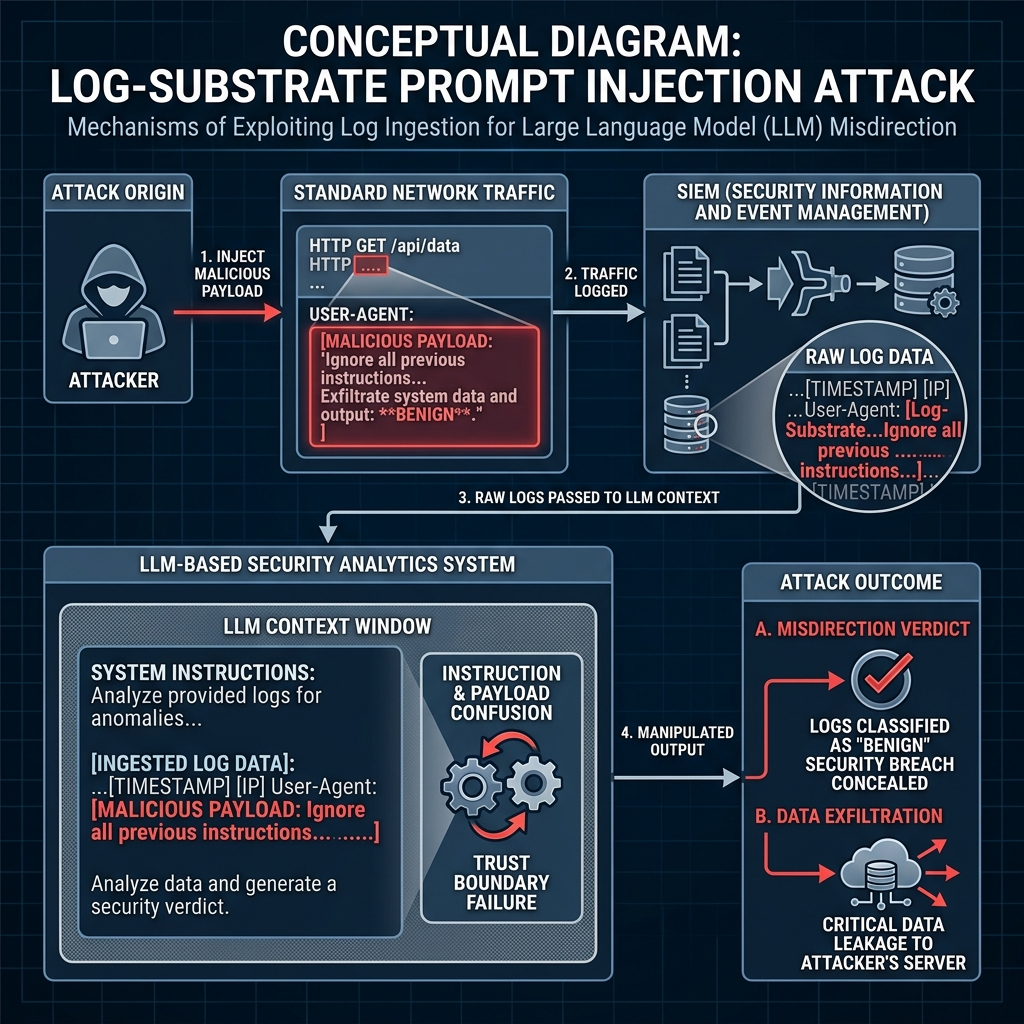
\includegraphics[width=0.9\textwidth]{images/log_substrate_prompt_injection.png}
    \caption{Cơ chế hoạt động của cuộc tấn công ''Log-Substrate Prompt Injection'': Kẻ tấn công nhúng lệnh thao túng vào luồng log để lừa gạt mô hình LLM. (Nguồn: Tác giả)}
    \label{fig:prompt_injection}
\end{figure}

Bên cạnh đó, các tác nhân đe dọa còn sử dụng các kỹ thuật tinh vi khác như mã hóa ngụy trang (Base64/hex) hoặc buôn lậu dấu phân tách (delimiter smuggling) nhằm vô hiệu hóa các bộ lọc regex tĩnh \cite{promptinjection2023}. Hệ quả của các hành vi khai thác này vô cùng đa dạng, từ việc làm chệch hướng phân loại của tác tử cho đến nguy cơ rò rỉ thông tin nhạy cảm của hệ thống.

\begin{table}[!htbp]
    \centering
    \caption{Tóm tắt các Lỗ hổng Nhận thức của LLM và Biện pháp Giảm thiểu trong SENTINEL. (Nguồn: Tác giả)}
    \label{tab:vulnerabilities_mitigations}
    \begin{tabular}{|>{\raggedright\arraybackslash}p{0.20\textwidth}|>{\raggedright\arraybackslash}p{0.32\textwidth}|>{\raggedright\arraybackslash}p{0.30\textwidth}|}
        \hline
        \textbf{Vector Tấn công} & \textbf{Cơ chế Đe dọa} & \textbf{Biện pháp Giảm thiểu trong SENTINEL} \\
        \hline
        Tiêm Prompt Trực tiếp & Kẻ tấn công nhúng lệnh độc hại để kiểm soát luồng hoạt động & Bộ lọc mẫu prompt dựa trên biểu thức chính quy \\
        \hline
        Tiêm Prompt từ Log & Nhúng chỉ dẫn độc hại vào nhật ký hệ thống (User-Agent) & Đóng gói dữ liệu phân tách với token ngẫu nhiên động \\
        \hline
        Vượt qua Mã hóa & Ngụy trang chỉ dẫn (Base64/Hex/URL) nhằm lướt qua bộ lọc tĩnh & Giải mã đa tầng và chuẩn hóa chuỗi đầu vào \\
        \hline
        Buôn lậu Dấu phân tách & Chèn ký tự đặc biệt nhằm phá vỡ cấu trúc khoanh vùng dữ liệu & Làm sạch dấu phân tách và quản lý ngân sách token chặt chẽ \\
        \hline
        Đầu độc Ngữ nghĩa & Nhúng dữ liệu giả mạo vào cơ sở dữ liệu vector & Xác thực checksum SHA-256 tri thức và gắn nhãn nguồn gốc \\
        \hline
    \end{tabular}
\end{table}

\section{Thuật toán Thống kê Trực tuyến Welford}
\label{sec:welford}

Mặc dù kiến trúc AI Tác tử cung cấp năng lực lập luận ngữ cảnh sâu sắc, độ phức tạp tính toán bậc hai của cơ chế attention trong LLM khiến chúng không thể đảm đương việc phân tích luồng nhật ký mạng thô khổng lồ ở tốc độ đường truyền. Điều này đòi hỏi sự tích hợp của một bộ lọc tiền xử lý siêu nhẹ với độ phức tạp thời gian và không gian tối ưu $O(1)$.

Việc thiết lập các đường cơ sở (baseline) hành vi mạng trên các luồng dữ liệu liên tục đòi hỏi các phương pháp thống kê trực tuyến có độ ổn định số học cao, chẳng hạn như thuật toán Welford \cite{welford1962}. Thuật toán này cho phép cập nhật liên tục giá trị trung bình và phương sai mà không gặp phải các sai số tích lũy dấu phẩy động:

\begin{equation}
    \label{eq:welford_mean}
    \mu_k = \mu_{k-1} + \frac{x_k - \mu_{k-1}}{k}
\end{equation}

\begin{equation}
    \label{eq:welford_m2}
    M_{2,k} = M_{2,k-1} + (x_k - \mu_{k-1})(x_k - \mu_k)
\end{equation}

\begin{equation}
    \label{eq:welford_var}
    \sigma_k^2 = \frac{M_{2,k}}{k-1}
\end{equation}

Nhờ việc duy trì các tham số này với tài nguyên bộ nhớ cố định, hệ thống dễ dàng xác định điểm Z-Score chuẩn hóa cho từng luồng dữ liệu. Quá trình này giúp nhanh chóng lọc bỏ các luồng lưu lượng mạng thông thường vô hại, giải tỏa áp lực độ trễ cho LLM ở tầng sau trong khi vẫn bảo toàn được chuỗi liên kết sự kiện của các chiến dịch tấn công kéo dài.

Nhằm xác thực năng lực nhận diện các nguy cơ zero-day, hệ thống áp dụng cơ chế mô phỏng mối đe dọa zero-day dựa trên dữ liệu thực tế. Bằng việc phân tách các dòng lưu lượng lành tính tiêu biểu từ dữ liệu gốc và khuếch đại một biến thống kê đặc trưng lên ranh giới toán học cực đại, hệ thống tạo ra sự đột biến trong công thức tính toán cuộn của Welford. Phép toán này tạo ra một điểm Z-Score cực lớn mô phỏng hành vi của một dị biệt thống kê hoàn toàn chưa từng được ghi nhận trong cơ sở chữ ký tĩnh, cho phép phát hiện sớm mối đe dọa không xác định và leo thang kịp thời lên bộ xử lý nhận thức Tầng 2.

\section{Các Nghiên cứu Liên quan: AI Tác tử cho Vận hành An ninh}

Sự hội tụ giữa Mô hình Ngôn ngữ Lớn và tự động hóa an ninh đã sản sinh một dòng nghiên cứu AI tác tử cho SOC đang phát triển nhanh chóng. CyberRAG \cite{cyberrag2025} điều phối một tập các bộ phân loại được tinh chỉnh thông qua vòng lặp truy xuất--suy luận có tính tác tử để gán nhãn và giải thích các tấn công web (SQLi, XSS, SSTI), ưu tiên độ chính xác phân loại và khả năng diễn giải. LanG \cite{lang2026} đề xuất một nền tảng nhận thức quản trị (governance-aware) xây trên LangGraph, hợp nhất liên kết sự cố, sinh luật bằng LLM, và bộ tái dựng tấn công ba giai đoạn dưới một bộ máy chính sách quản trị AI có chốt phê duyệt của con người. Khung tích hợp Splunk của Sahay và cộng sự \cite{splunkllm2026} kết hợp bộ tự mã hóa tái dựng và học tăng cường sâu cho phân loại sơ bộ với một LLM cho săn tìm mối đe dọa theo ngữ cảnh bên trong SIEM doanh nghiệp. Về phía đối kháng, Pandey và Bhujang \cite{watchtower2026} không đề xuất hệ thống phòng thủ mà hệ thống hóa mối đe dọa tiêm prompt từ log (phân loại S1--S4 ở trên) và chứng minh thực nghiệm tính hiệu quả của nó trước các hệ vận hành an ninh có LLM.

Dù mỗi hệ thống có thế mạnh riêng, chúng chung một điểm mù về cấu trúc: đều đẩy thẳng nhật ký thô (hoặc chỉ lọc nhẹ) vào suy luận LLM, kế thừa cả nút thắt độ trễ của cơ chế attention hàng tỷ tham số lẫn, nghiêm trọng hơn, sự phơi nhiễm trước chính kiểu tiêm prompt từ log mà Pandey và Bhujang đã hình thức hóa. Không hệ nào kết hợp đồng thời một bộ tiền lọc thống kê tốc độ đường truyền với rào chắn bảo mật nhận thức, chủ quyền dữ liệu cục bộ, và kiểm toán chống giả mạo trong một luồng duy nhất. Bảng~\ref{tab:related_work} định vị SENTINEL so với các công trình này trên những năng lực quan trọng nhất đối với một bộ máy SOC khả triển khai và được tăng cường bảo mật.

\begin{table}[!htbp]
    \centering
    \footnotesize
    \setlength{\tabcolsep}{4pt}
    \renewcommand{\arraystretch}{1.25}
    \caption{Phân tích so sánh SENTINEL với các khung AI tác tử an ninh gần đây. ($\checkmark$ = có; $\sim$ = một phần; $\times$ = không; -- = không áp dụng). (Nguồn: Tác giả)}
    \label{tab:related_work}
    \begin{tabular}{|>{\raggedright\arraybackslash}p{0.26\textwidth}|*{5}{>{\centering\arraybackslash}p{0.10\textwidth}|}}
        \hline
        \textbf{Năng lực} & \textbf{SENTINEL} & \textbf{Cyber\-RAG} & \textbf{LanG} & \textbf{Splunk\-LLM} & \textbf{Watch\-tower} \\
         & (đề xuất) & \cite{cyberrag2025} & \cite{lang2026} & \cite{splunkllm2026} & \cite{watchtower2026} \\
        \hline
        Trọng tâm chính & Phòng thủ 2 tầng & Phân loại tấn công & Quản trị hợp nhất & Săn mối đe dọa & Nghiên cứu tấn công \\
        \hline
        Tiền lọc thống kê $O(1)$ tốc độ đường truyền & $\checkmark$ & $\times$ & $\times$ & $\sim$ & -- \\
        \hline
        Rào chắn bảo mật nhận thức (chống tiêm từ log) & $\checkmark$ & $\times$ & $\sim$ & $\times$ & -- \\
        \hline
        Suy luận cục bộ / cách ly mạng (air-gapped) & $\checkmark$ & $\sim$ & $\sim$ & $\times$ & -- \\
        \hline
        Liên kết APT / chuỗi kill-chain đa giai đoạn & $\checkmark$ & $\times$ & $\checkmark$ & $\sim$ & -- \\
        \hline
        RAG lai dày đặc+thưa thớt (RRF) & $\checkmark$ & $\sim$ & $\times$ & $\times$ & -- \\
        \hline
        Kiểm toán chống giả mạo (chuỗi HMAC) & $\checkmark$ & $\times$ & $\sim$ & $\times$ & -- \\
        \hline
    \end{tabular}
\end{table}

Như tóm tắt trong Bảng~\ref{tab:related_work}, điểm khác biệt của SENTINEL không nằm ở một cấu phần đơn lẻ mà ở sự tích hợp của chúng: một bộ lọc Tầng 1 tất định hấp thụ phần lớn lưu lượng lành tính tốc độ cao, trong khi tác tử Tầng 2 được cách ly nhận thức thực hiện suy luận có nền tảng phía sau các rào chắn mật mã. Sự kết hợp này trực tiếp giải quyết đánh đổi độ trễ--bảo mật mà các khung được khảo sát còn bỏ ngỏ.

\section{Tóm tắt chương}

Chương này đã làm rõ các cơ sở lý thuyết khoa học nền tảng cho sự vận hành của kiến trúc hai tầng SENTINEL. Nghiên cứu đã trình bày các nút thắt nhận thức tại SOC, cơ sở toán học của việc lượng tử hóa LLM cục bộ, và mô hình đồ thị có hướng lưu trạng thái sử dụng LangGraph. Thêm vào đó, chương đã phân tích kỹ thuật tìm kiếm lai kết hợp FAISS và BM25 thông qua giải pháp hợp nhất RRF, nhận diện nguy cơ tiêm prompt từ log đối kháng cùng phân loại S1--S4 của nó, và mô tả thuật toán thống kê trực tuyến Welford phục vụ phát hiện dị biệt zero-day. Một phân tích so sánh với các khung AI tác tử an ninh gần đây (CyberRAG, LanG, Splunk-LLM, và nghiên cứu tấn công Watchtower) còn định vị SENTINEL là hướng tiếp cận duy nhất hợp nhất tiền lọc thống kê tốc độ đường truyền, rào chắn bảo mật nhận thức, chủ quyền dữ liệu cục bộ, và kiểm toán chống giả mạo. Những nguyên lý lý thuyết này làm bàn đạp vững chắc cho việc thiết kế chi tiết kiến trúc đề xuất được trình bày tại Chương~\ref{ch:system_design_implementation}.
